% if there are questions please contact me:
% karsten.rink@ufz.de

%\newcommand{\ogs}{OpenGeoSys }

\chapter{Data processing}
\textit{by Karsten Rink and Thomas Fischer}

\bigskip

\ogs is a program for the simulation of (coupled) thermal, hydrological, mechanical and chemical processes that contains large amount of FEM-related functionality and numerical solvers. It is, however, a command line tool and therefore not intuitive to handle for first time users. Also, it is difficult to get a feeling for the data that is utilized by the program and simulation results cannot be directly verified without the help of other tools.

To address these issues, the \ogs Data Explorer has been developed as a graphical user interface (GUI) for \ogs (see fig. \ref{fig:kr:gui}). This allows for a 3D visualization of input and output data of process simulations and will thus convey a better understanding of the data as well as the simulations. As with the simulation software itself, the Data Explorer is platform independent due to the use of the open source application framework Qt and is tested under Windows- and Linux-based operating system as well as MacOS. It employs the same basic data structures as the command line tool and thus complements \ogs by giving users a way to visually assess their data sets.

\begin{figure}[tb]
\begin{center}
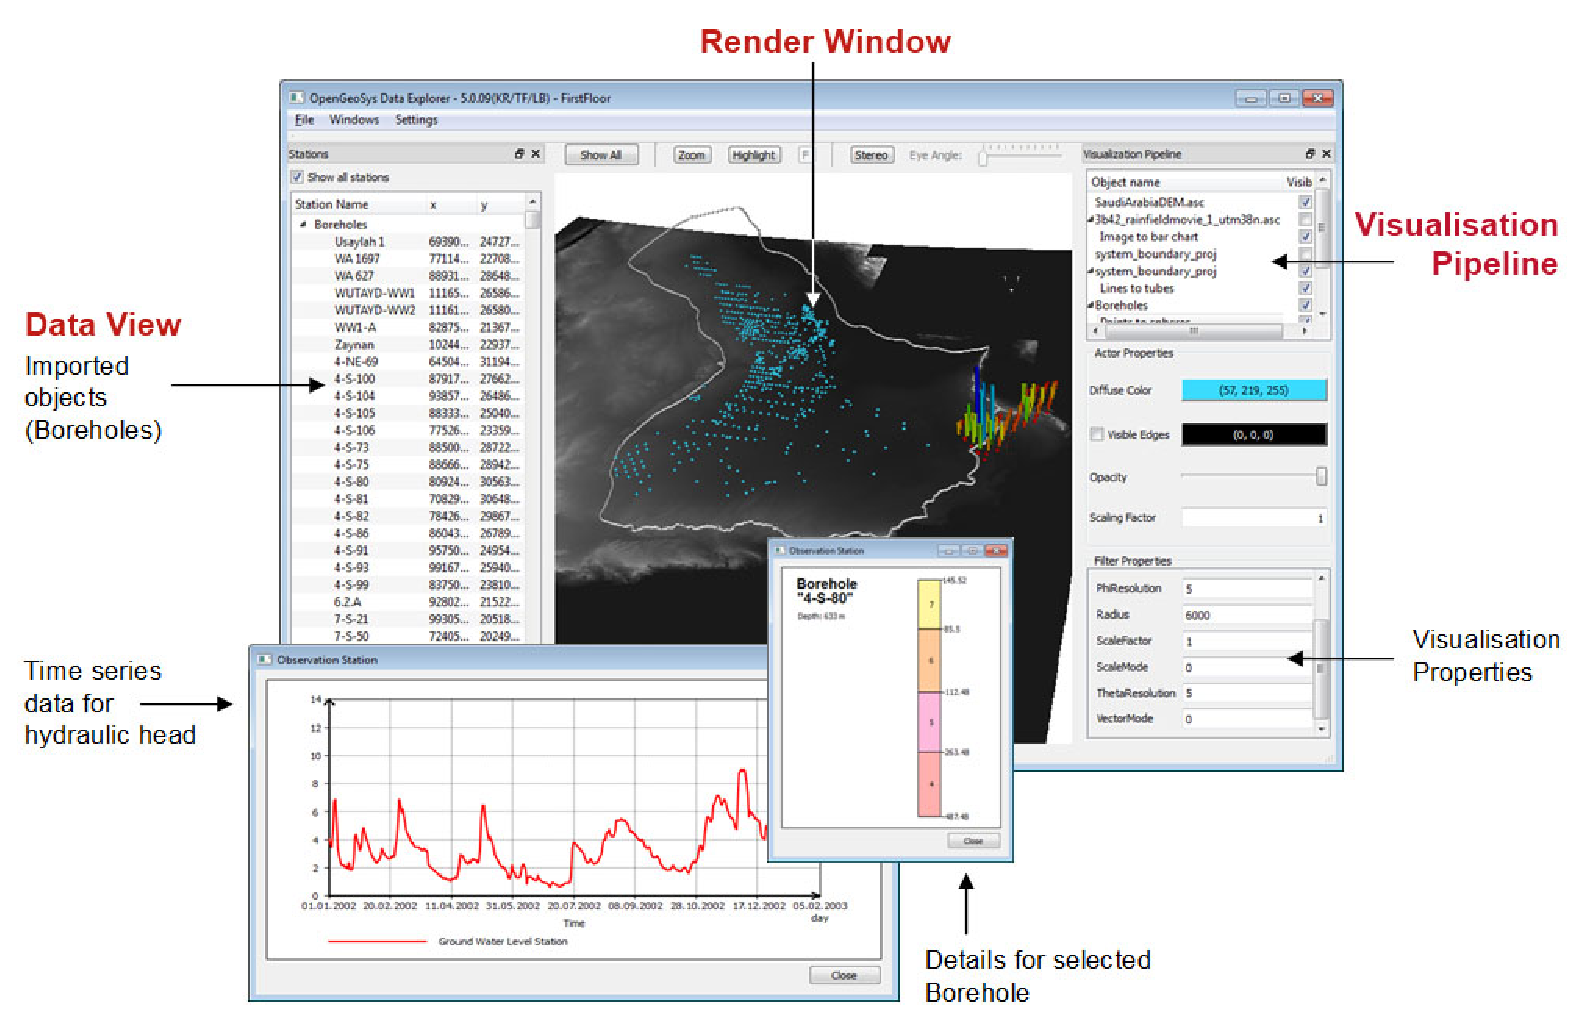
\includegraphics[width=0.99\linewidth]{figures/gui}
\caption{The graphical user interface of the \ogs Data Explorer.}
\label{fig:kr:gui}
\end{center}
\end{figure}

An interactive 3D view (see fig. \ref{fig:kr:vis}) often enhances the understanding of the data and makes it easier to discuss certain aspects or problems with other scientists. Besides handling the native \ogs file formats, the Data Explorer also provides a large number of interfaces for the import of files created by established geoscientific software products such as the geographic information system ArcGIS, the groundwater modeling software GMS and -- to a certain degree -- software used in the mining or petroleum industry such as Petrel or Gocad. Non-spatial information such as time series data or borehole stratigraphies can be viewed in separate 2D windows. Furthermore, it is possible to import image data in popular formats such as JPEG or PNG. In addition to all these geoscientific input data formats, it is also possible to visualize FEM-related information like boundary conditions (see fig. \ref{fig:kr:cond}) and  or 3D object structures in the widespread VTK format. In particular, this format is used to store the time invariant results of process simulations calculated using \ogs.

The Data Explorer supports users when preparing simulations of processes by allowing them to see how various data sets complement or interact with each other. When data sets from various sources are used, it is not uncommon that inconsistencies between those data sets exist. Typical examples in the scope of hydrological data include the course of rivers not quite matching the underlying terrain model, subsurface layers penetrating each other or boreholes not starting at ground level but instead above or below the surface. The reasons for such inconsistencies are manifold and can be attributed to different data acquisition methods (such as remote sensing data scanned from orbit via satellites, borehole logs created manually using core samples, etc.), data conversion problems or human error.  However, if models for the simulation of processes such as groundwater recharge are based on faulty or conflicting information they might produce erroneous or deceptive results. An interactive 3D view allows the user to assess the quality of the data and detect inconsistencies, artifacts or missing information.

\begin{figure}[tb]
\begin{center}
\subfigure[2D view]{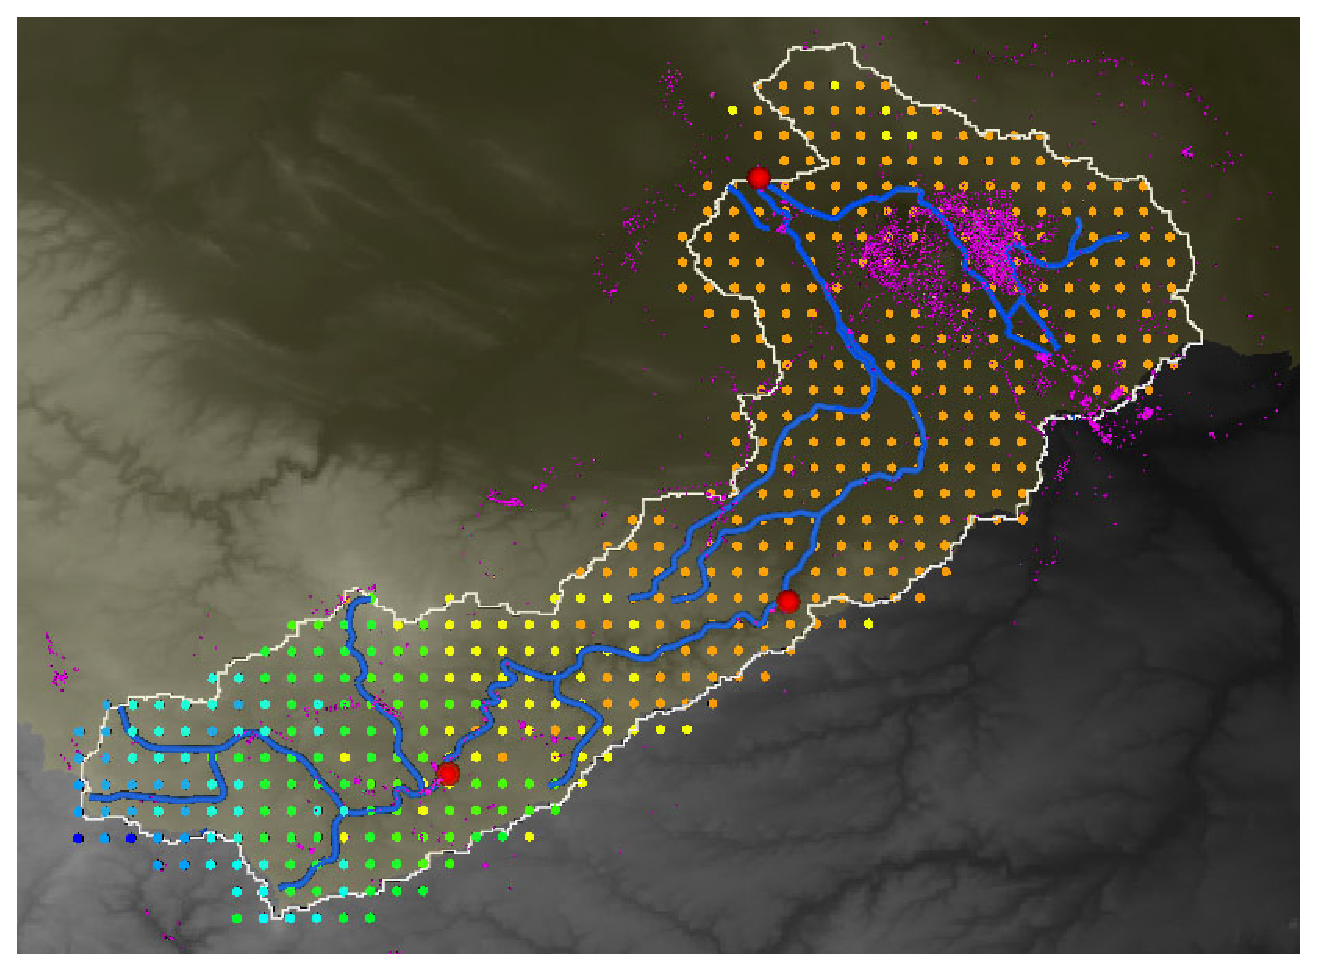
\includegraphics[width=0.48\linewidth]{figures/DEMSelke}\label{fig:kr:selke2d}}\enspace
\subfigure[3D view]{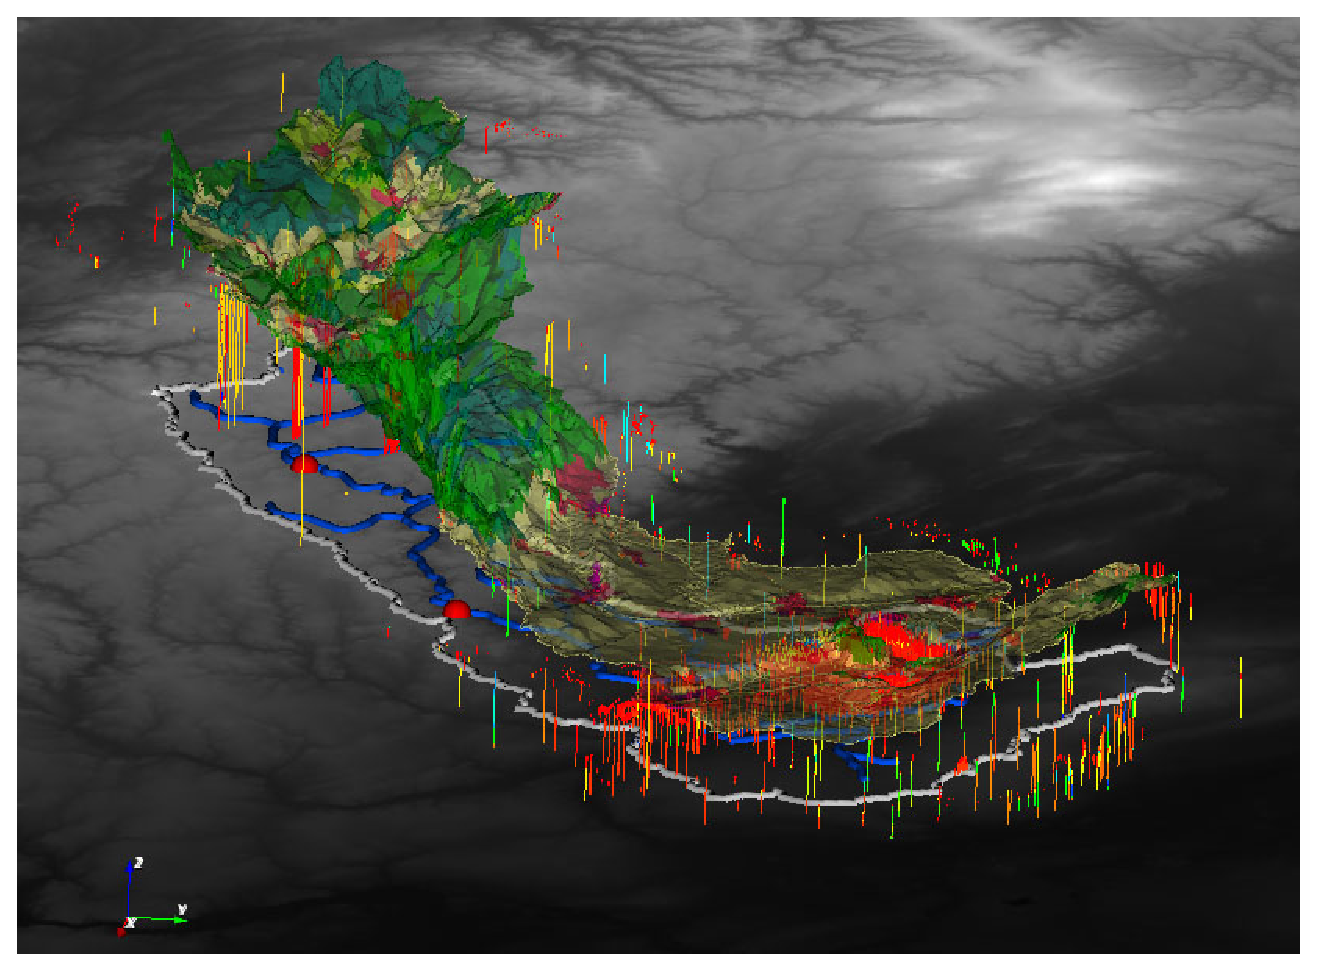
\includegraphics[width=0.48\linewidth]{figures/DEMSelke3D}\label{fig:kr:selke3d}}
\end{center}
\caption{Example for visualization of multiple data sets. Figure \ref{fig:kr:selke2d} depicts geometrical information such as the boundary of the model region (white), the river network (blue), gauging stations (red) and boreholes (pink) in addition to a discrete precipitation map where the blue dots mark high precipitation and the red/orange dots low precipitation. Figure \ref{fig:kr:selke3d} shows the same scene in 3D (although without the precipitation). Boreholes can now be seen as 3D structures. A semi-transparent surface mesh overlaid with land use classes as been added to the scene.} \label{fig:kr:vis}
\end{figure}

\begin{figure}[tb]
\begin{center}
\subfigure[Information]{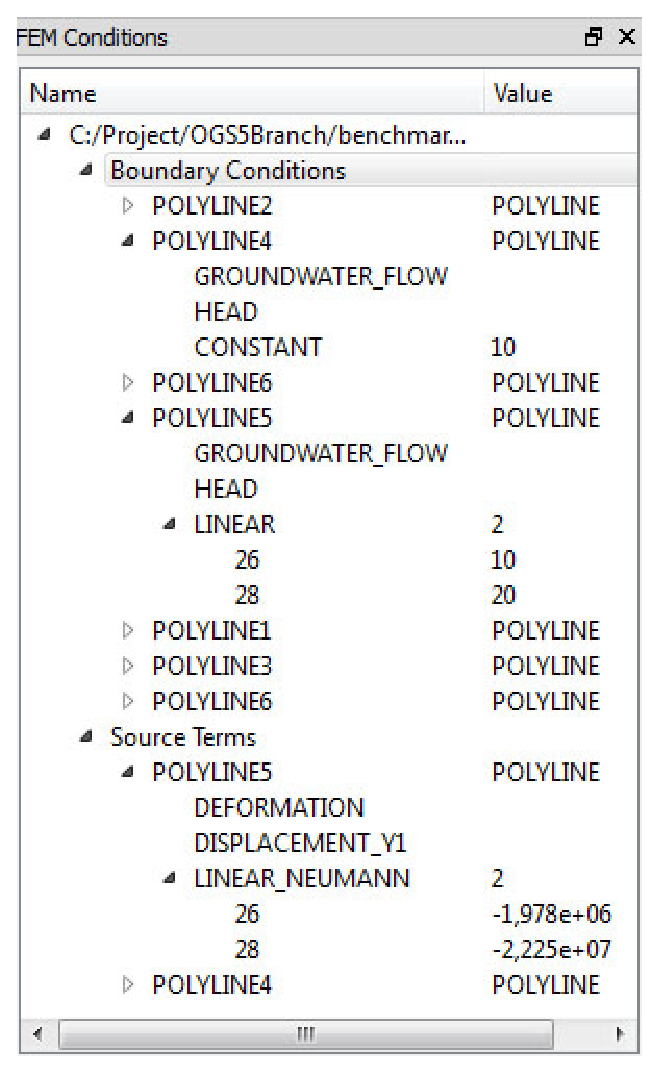
\includegraphics[width=0.33\linewidth]{figures/gui_cond_menu}\label{fig:kr:condmenu}}\enspace
\subfigure[3D visualization]{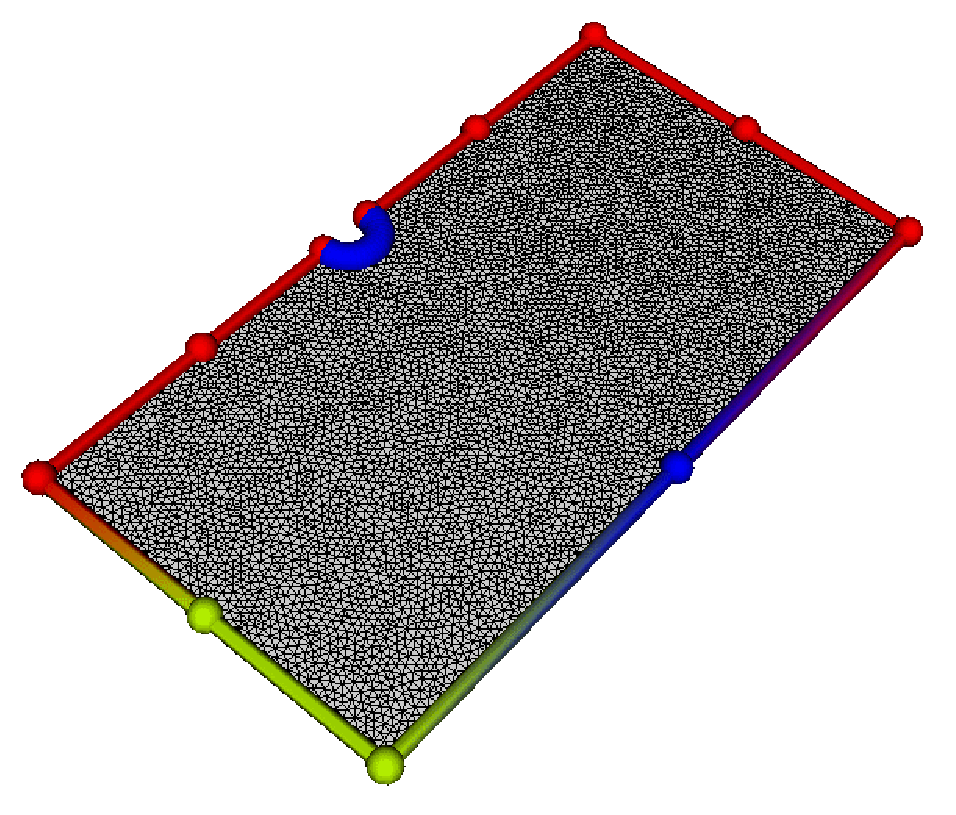
\includegraphics[width=0.65\linewidth]{figures/gui_cond_vis}\label{fig:kr:condvis}}
\end{center}
\caption{Example for visualisation of FEM related data. Depicted are a number of boundary conditions for a FEM Mesh along with detailed information about their properties.} \label{fig:kr:cond}
\end{figure}

A number of visualization options are available in the GUI to support users in this assessment process by allowing the adjustment of a number of visualization parameters for each data set. Examples include

\begin{itemize}\addtolength{\itemsep}{-0.3\baselineskip}
\item Super elevation of objects
\item Adjusting transparency, such that objects occupying the same space can be evaluated
\item Application of user defined color tables (e.g. for borehole information)
\item Selection of specific materials or stratigraphic layers (e.g. a specific set of lines or a certain subsurface layer) while blanking out the rest of the data set.
\item Enlargement of selected features for better visibility
\end{itemize}

In addition, users can see the underlying data of visualized objects (such as point coordinates, mesh element information, etc.) in a separate menu and can even process geometric data to a certain degree (connecting polylines, triangulation of surfaces, etc.). Furthermore, it is possible to generate parameterized FEM meshes based on existing geometric data with a desired element density and optional mesh refinement towards selected features. For existing meshes it is possible to check the quality of all mesh elements with respect to certain well-establish criteria such as the ratio of longest to shortest element edge, equi-angle skewness or global element area/volume and then analyze the results of such an analysis directly in the 3D view (see fig. \ref{fig:kr:meshqual}).

\begin{figure}[!b]
\begin{center}
\subfigure[All elements]{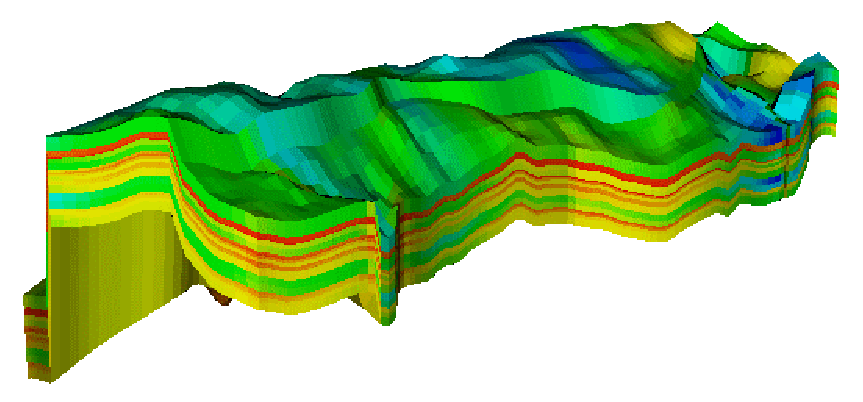
\includegraphics[width=0.48\linewidth]{figures/meshqual1}\label{fig:kr:meshqual1}}\enspace
\subfigure[Zero volume elements]{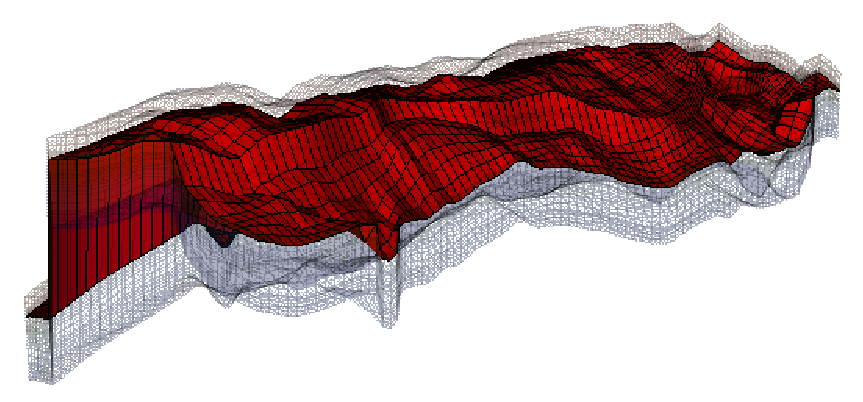
\includegraphics[width=0.48\linewidth]{figures/meshqual2}\label{fig:kr:meshqual2}}
\end{center}
\caption{Visualization of mesh element quality. Blue signifies good quality, red elements might cause problems during simulation. Figure \ref{fig:kr:meshqual2} depicts a layer containing zero volume elements blended into the transparent mesh.} \label{fig:kr:meshqual}
\end{figure}

%The \ogs Data Explorer is being actively developed at the Helmholtz Centre for Environmental Research and regular updates introduce new features for the handling and visualization of data.

For more information on the topic of evaluation of 3D data sets the interested reader is referred to \cite{rink:cgvcvip2011}. A comprehensive specification of the functionality of the \ogs Data Explorer can be found in %the \emph{OpenGeoSys Data Explorer User Manual}
\cite{rink:manual}.
